\section{CALIBRATION}

\begin{yellowbox}{\textbf{NOMENCLATURE}}
    \begin{tabularx}{\columnwidth}{ll}
        $$ & \\
        \addlinespace[2pt]
        $$ & \\
        $$ & \\
        $$ & \\
        $$ & \\
        $$ & \\
        $$ & \\
        $$ & \\
        $$ & \\
   
    \end{tabularx}
\end{yellowbox}

\begin{whitebox}{\textbf{CONFIDENCE CALIBRATION}}
    \begin{itemize}
        \item Problem of predicting probability estimates representative of the true correctness likelihood
        \item Goal of calibration: align probabilities with their true correctness likelihood
        \item Calibration will compromise accuracy (except for temperature scaling)
        \item Well calibrated: confidence region $\mu\pm\sigma$ includes all true data points
    \end{itemize}
\end{whitebox}

\begin{whitebox}{\textbf{RELIABILITY DIAGRAMS}}
    \begin{center}
        \resizebox{0.95\linewidth}{!}{
            \includegraphics[
            page=32,
            trim = {7.7cm, 1.9cm, 0.1cm, 5.17cm}, % left, bottom, right, top
            clip
            ]{media/23HS_Tut07_BDL.pdf}
        }
    \end{center}
    \begin{itemize}
        \item Expected sample accuracy as a function of confidence
        \begin{enumerate}
            \item Predictions grouped into $M$ interval bins of size $\frac{1}{M}$
            \item Calculate relative frequency of positive samples for each bin
            \begin{align*}
                \mathrm{freq}(B_m)=\frac{1}{|B_m|}\sum_{i\in B_m}\bm{1}(\hat{y}_i=1)
            \end{align*}
            where $B_m$ is the set of samples falling into bin $m$
            \item Calculate the average confidence within the bin
            \begin{align*}
                \mathrm{conf}(B_m)=\frac{1}{|B_m|}\sum_{i\in B_m}\hat{p}_i
            \end{align*}
        \end{enumerate}
    \end{itemize}
\end{whitebox}

\begin{whitebox}{\textbf{CALIBRATION METHODS}}
    \begin{itemize}
        \item Empirically improve accuracy of calibration via heuristics
        \begin{itemize}
            \item Histogram binning
            \begin{enumerate}
                \item Divide uncalibrated predictions $\hat{p}_i$ into bins $B_1,\dots,B_M$
                \item Assign calibrated score to each bin
                \begin{align*}
                    \hat{q}_i=\mathrm{freq}(B_m)
                \end{align*}
            \end{enumerate}
            \item Isotonic regression
            \begin{itemize}
                \item Find piecewise constant function $f:\hat{q}_i=f(\hat{p}_i)$ that minimizes the bin-wise squared loss
                \begin{align*}
                    \min_{M,\theta_1,\dots,\theta_M,a_1,\dots,a_{M+1}}\sum_{m=1}^M\sum_{i=1}^n\mathbf{1}(a_m\leq\hat{p}_i<a_{m+1})(\theta_m-y_i)^2
                \end{align*}
                subject to
                \begin{align*}
                    0=a_1\leq a_2\leq&\dots\leq a_{M+1}=1\quad\text{(bin boundaries)}\\
                    \theta_1\leq\theta_2\leq&\dots\leq\theta_M\quad\text{(values in each bin)}
                \end{align*}
            \end{itemize}
            \item Platt scaling
            \begin{itemize}
                \item Learn parameters $a,b\in\mathbb{R}$ that minimize the NLL loss over the validation set when applied to the logits $z_i$
                \begin{align*}
                    \hat{q}_i=\sigma(az_i+b)
                \end{align*}
                \item Temperature scaling
                \begin{align*}
                    &b=0\\
                    &a=\frac{1}{T}
                \end{align*}
                \begin{itemize}
                    \item Higher temperature $\to$ softer probabilities
                    \item Lower temperature $\to$ sharper probabilities
                \end{itemize}
            \end{itemize}
            \item BNNs often improve calibration in practice \textit{without} any heuristics applied
        \end{itemize}
    \end{itemize}
\end{whitebox}

\begin{whitebox}{\textbf{TWO TYPES OF UNCERTAINTY}}
    \begin{itemize}
        \item Epistemic uncertainty
        \begin{itemize}
            \item Model uncertainty that corresponds to uncertainty in model parameters and can be explained away given enough data
        \end{itemize}
        \item Aleatoric uncertainty
        \begin{itemize}
            \item Inherent noise in observations
            \begin{itemize}
                \item Homoscedastic noise: independent of input
                \item Heteroscedastic noise: dependent on input
            \end{itemize}
        \end{itemize}
        \faWarning\ Uncertainties depend on the data \textit{and} the model (e.g. a linear model would interpret nonlinearities as noise)
    \end{itemize}
\end{whitebox}